\documentclass[a4paper,10pt]{article}

% abstract + title + authors
\usepackage{abstract}
\renewcommand{\abstractnamefont}{\normalfont\bfseries}
\renewcommand{\abstracttextfont}{\normalfont\small\itshape} 
\usepackage{titlesec}
\usepackage{authblk}
\usepackage{datetime}
\newdateformat{usvardate}{
\monthname[\THEMONTH] \ordinal{DAY}, \THEYEAR}

% keywords
\providecommand{\keywords}[1]{\textbf{\textit{Keywords---}} #1}

% math
\usepackage{amssymb}
\usepackage{newtxmath}

% manuscript looking document
\usepackage{setspace}
\usepackage{lineno,xcolor}
\setlength{\parskip}{0.5em}

% comments

% graphics
\usepackage{graphicx}
\usepackage{float}

% references & links
\usepackage{hyperref}
\hypersetup{
    colorlinks=true,
    citecolor=magenta,
    linkcolor=magenta
}
 % See preamble.tex to edit the overall layout

\usepackage{Sweave}
\begin{document}
\Sconcordance{concordance:manuscript.tex:/Users/efc29/github/driver-species/paper/manuscript.Rnw:%
1 47 1 1 0 29 1 1 7 23 1 1 9 1 2 10 1 1 26 1 2 8 1 1 18 1 2 10 1 1 36 1 %
2 4 1 1 33 1 2 18 1 1 9 1 2 27 1}

\setkeys{Gin}{width=1\textwidth}

% title
% Article title
  \title{\fontsize{16pt}{10pt}\selectfont\textbf{Structural controlability of pollination networks}}

% Authors and Affiliations
  \author[1]{\large E. Fernando Cagua}
  \author[1]{\large Daniel B. Stouffer}
  \affil[1]{\normalsize Center of Integrative Ecology, School of Biological Sciences, University of Canterbury}
 
 \date{\small\usvardate\today}

\maketitle

\begin{abstract}
\noindent Si sabemos que el disfrute exige lentitud, y que---mas en general---la felicidad se asocia con el ir despacio, por que corremos tanto? El arte de comer estriba en saborear cada bocado sin pensar en el siguiente, sin apresurar el siguiente. El arte de leer, en demorarse en cada palabra como si el sentido del escrito entero estuviera contenido en ella. El arte de amar, en vivir cada momento de la relacion con la persona amada como si fuese el destino de toda la historia del mundo, desde la aparicion del primer organismo unicelular hasta hoy. Y asi podemos generalizar a las demas actividades, creo, hasta obtener un arte de vivir. Para mi se resume en la palabra ahi. --- Jorge Riechmann
\end{abstract}

\keywords{Control theory}

% line numbers
\linenumbers
\setlength\linenumbersep{15pt}
\renewcommand\linenumberfont{\normalfont\footnotesize\sffamily\color{gray}}

\onehalfspacing


% Main Text
\section*{Introduction}

Ecological communities are formed by the interconnection of several species. Therefore, changes in the abundances of one species can potentially alter the abundances of the species they interact with. For instance, in a classic example of ecosystem cascades, a reduction on the abundance of sea otters, an important predator or sea urchins, can drive a dramatic reduction on kelp abundances because the sea urchins that consume kelp are released from predation. It has been long established that some species, like the sea otter, have a disproportionate large effect in their environment relative to their abundance. 

In several ecosystems the relative importance of species have been identified based on empirical observations of long term dynamics. However, in less studied, highly diverse, or where the "keystone" role is shared by several species, it can be challenging to determine which is the set of species that influence the most the ecosystem dynamics. Alternative approaches that recognize a continuum of importance and that are less dependent on empirical observations have also been developed. Some of them are based on metrics that evaluate their position in the food web or on mass balance models of functional groups. Nevertheless, these approaches are conceptually limited to throphic interactions and in general ignore the structural mechanisms that allow or prevent the spread of perturbations in the ecosystem.

From a systems perspective, perturbations like over-exploitation, eutrophication or global warming are equivalent to management actions like culling, no-take areas or captive rearing in the sense that they have the potential to modify the abundances of one or several species in the ecosystem. Therefore identifying these key species is crucial not only to predict how these perturbations will spread trough the community but also to guide effective conservation efforts.

Recent work on the control of complex systems suggest that in principle it is possible to alter any ecological community's composition, by modifying the abundances of just some key species. Here, we apply these theories to estimate the controllability of different ecological communities and to find the species, that due to the structural characteristics of their interactions are more likely to drive the dynamics of the community. 

\section*{Methods \& Results}

Using six paired plant pollinator communities we explored the concepts of control theory. This is the initial data set things will be tested. If more data is considered necessary we'll see that later. 

\subsection*{Controllability of ecological communities}

\subsubsection*{Minimum set of species } 

Using maximum matching to control all species in the network. We found that depending on the scheme around of the species are needed to have a grasp at the whole community (\autoref{fig:n_species}). However, the relative ranking of networks remains relatively unchanged across schemes. So rather than focusing on the differences across schemes perhaps it would be interesting to see what characteristics make a network to require more or less driver nodes to be completely controled. Alternatively it would be interesting to see if there are systemic differences between different types of networks. An initial step would be to stay with bipartite networks of the mutualistic type (plant/frugivores) or the the consumer-resource type (host/paraiste or predator/prey). Perhaps some model networks of varying parameters?

\begin{figure}
\centering
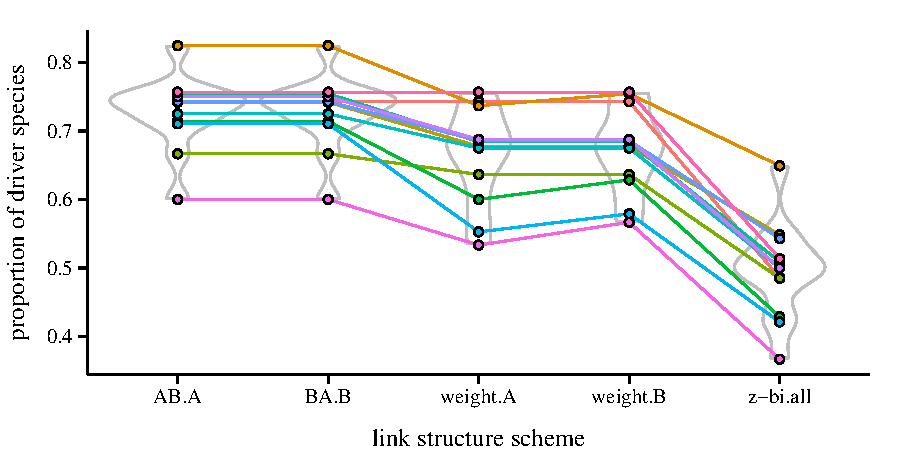
\includegraphics{figures/fig--002}
\caption{\label{fig:n_species} Proportion of species that needs to be controled for all twelve networks under different link assumptions. AB indicates that the links go from plants to pollinators; BA that the links go from pollinator to plants; ``weight'' that the direction of control is chosen by dependency (ties are resolved by giving priority to plants in weight.A and to pollinators in weight.B); z-bi indicates that the links go in both directions}
\end{figure}

\subsubsection*{Profiles of critical and redundant species}

Dividing the nodes and links among critical, ordinary and redundant we can have an idea of ``control profiles'' of the networks. 

\subsubsection*{Profiles of internal/external dilation}

\subsection*{Ranking species}

By frequency in control sets

Strongly interacting species (interaction heterogeneity)

\section*{Discussion}

 For instance, restoration projects that aim to drive an invasive species out of the community, to reestablish a particular ecosystem service or in general modify the ecosystem state have had a limited amount of success. We argue that quantifying the relative dynamic importance of species the set of key species is the first step to evaluate current management efforts as well as to design targeted and informed 
 
 Dynamic system approach
 
\section*{Acknowledgmenets}

Takeuki Uno for the insight provided to find the set of all maximum matching algorithms.


\end{document}
